\section{Introduction}
\label{sec:intro}

LiDAR--inertial odometry (LIO) combines inertial propagation with corrections
from scan registration. This propagation requires gravity and accelerometer
bias, but systems differ in whether these quantities remain estimated states
after initialization. FAST-LIO2 and Point-LIO retain gravity direction on $S^2$ online
\cite{xu2022fastlio2,he2023pointlio}, whereas LIO-SAM fixes it
\cite{shan2020liosam}. Lightning-LM goes further, reducing its filter from
23D to 12D by removing online estimation of accelerometer bias $\mathbf b_a$,
gravity $\mathbf g$, and the extrinsics \cite{gao2026lightninglm}. These designs
raise a practical question: which states need to remain online, and under
what operating conditions?

Comparing published trajectory errors cannot answer this question. The systems
also differ in registration, maps, trajectory models, and parameter settings. Even within
one system, a changing gravity estimate does not establish that estimating it
improves pose. Under weak excitation, changes in gravity, attitude, and
accelerometer bias can explain similar inertial residuals. Gravity may then
wander while LiDAR corrections keep the trajectory accurate. Removing gravity
could suppress this behavior, but could also remove an adjustment needed after
poor initialization or a long interruption of LiDAR correction.

Gravity adds only two tangent coordinates, so removing it offers little
computational incentive if point-cloud matching dominates runtime. The stronger
reason to fix gravity would be fewer weakly observable states without losing
accuracy or recovery. Testing that argument requires conditions beyond nominal
operation, where frequent scans may conceal the consequences of either choice.

We test whether online gravity estimation remains necessary for accurate pose
estimation when LiDAR updates are frequently accepted. We then weaken the available geometry
or remove corrections altogether to determine whether these conditions have
the same effect. Dynamic startup tests a different source of error: motion
during the shared acceleration-mean initialization. Keeping $\mathbf g$ and
$\mathbf b_a$ online permits subsequent adjustment, although their individual
estimates need not become physically correct. The experiments distinguish
improved trajectory estimation from accurate identification of these two
coupled quantities.

\begin{figure}[!t]
\centering
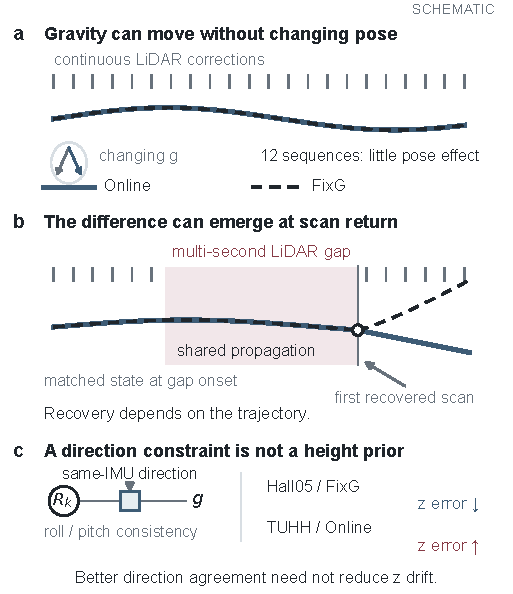
\includegraphics[width=\columnwidth]{figs/fig_teaser.pdf}
\caption{Study logic (schematic, not measured paths). \textbf{a}, Continuous
LiDAR correction can mask gravity-state motion. \textbf{b}, Matched states
share propagation; scan return can reveal different recovery.
\textbf{c}, A direction factor from the same IMU constrains attitude, not height:
the tested dropout cases show opposite vertical-error responses.}
\label{fig:teaser}
\end{figure}

Adding a gravity-direction factor is a separate design choice. Fixing gravity
removes a state, whereas the factor adds a residual that constrains attitude
relative to an estimated down direction. It does not measure height. Any
vertical-error reduction must arise indirectly through attitude, inertial
propagation, or scan registration. In particular, a direction estimate obtained
from the same IMU used for preintegration is not an independent observation.
We refer to this as a \emph{same-IMU direction factor}. We test whether closer
direction agreement lowers trajectory error, and whether the answer depends
on factor weight or on whether gravity is estimated online.

Runtime correction nulling cannot test state removal. Suppressed coordinates
remain in the covariance and influence retained variables through
cross-correlation. We instead compile four FAST-LIO2 state configurations,
each with a manifold that retains or removes gravity and accelerometer bias.
The front end, data, initialization, calibration, and parameter settings remain fixed. A true
$2\times2$ LIO-SAM state ablation provides a descriptive cross-architecture
check. Within that graph, factor on/off and fixed/online gravity isolate the
same-IMU direction factor.

Stress tests cover geometry degradation, periodic 1--5-s LiDAR absence, IMU
weighting, initialization error, and dynamic startup. A history-matched switch
separates fixing gravity from differences accumulated before an outage.
We report vertical position RMSE (RMSE$_z$) and 3D position RMSE (ATE), since
vertical improvement can accompany a worse trajectory. Absolute differences
help judge whether a large percentage change is practically important.

This work contributes:
\begin{itemize}
 \item within-system gravity and bias ablations in FAST-LIO2 and LIO-SAM,
 using actual state removal rather than suppressed corrections;
 \item tests of when state removal matters, including matched recovery after
 LiDAR outages and sensitivity to motion during initialization; and
 \item a direction-factor study showing that a smaller same-IMU residual
 does not guarantee lower vertical or 3D position error.
\end{itemize}

\noindent{\boldmath\textbf{Default: keep both $\mathbf g$ and $\mathbf b_a$
online. The tested same-IMU direction factor is not a generic $z$-drift remedy.}}
